%author: yjw, 2024-4-1
%\subsection{关键设计}
本项目核心目标是将自动模糊测试(Fuzzing)框架迁移到ROS2系统上,并且针对ROS2特性
对测试效率做出改进提升。具体而言,我们试图寻找更多可能的程序输入口,使测试覆盖的
输入可能性尽可能多;尝试构造质量尽可能高的测试用例;寻找更多反馈信息,用于监控被
测程序(即ROS2节点)的内部状态,以更高效地指导对输入的自动变异测试;尝试模拟更多
ROS2执行环境,模拟程序可能遇到的各种实际情况。

\subsubsection{通信环境测试}

如前所述,在机器人操作系统中,节点间通信方式可以基于本地网络套接字、有线通信、进
程内部通信等方式。在实际应用场景中,不能保证网路中通信的稳定性,如图\ref{pic:fmm}所
示,可能出现乱序、重复、丢包、变频等报文序列变化以及报文内容本身的变化。针对这一
观察,我们的ROS Fuzzer尝试对ROS2系统内部通信报文进行类似的变异,以测试ROS2程序的
鲁棒性。

\begin{figure}[h]
    \centering
    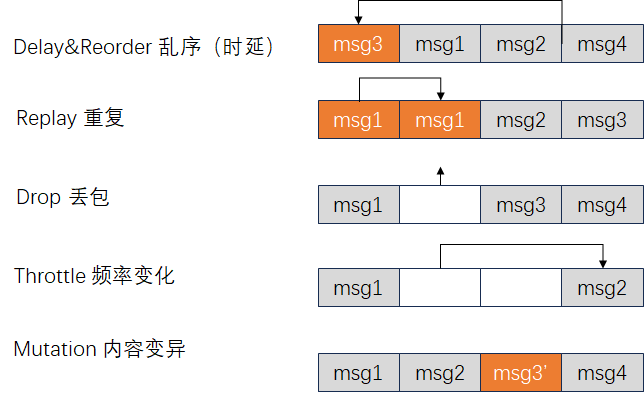
\includegraphics[width=10cm]{fuzz_msg_mutation.png}
    \caption{不稳定网路中的报文变化}
    \label{pic:fmm}
\end{figure}

已有测试框架Rozz$^{[2]}$建议在ROS2系统话题通信机制的订阅者和发布者建立恶意中介节
点,它会拦截消息发布者的消息,然后对消息进行变异后再转发给订阅者。本作品认为该方
案适用性有限,首先完全拦截消息难度大,尤其是对于节点内部硬编码的话题;其次ROS2抽
象层提供的QoS机制和时间戳机制能够过滤非法消息和保证通信质量,在ROS2上层进行消息
变异容易被识别为非法,不能较好模拟实际的网路不稳定性。

ROS2系统支持使用不同的DDS协议中间件实现,如Fast-DDS、Cyclone-DDS等,从而灵活适配
不同的需求。利用这一点,本作品创新性地用魔改的DDS通信中间件替代原有基础DDS中间
件,如图\ref{pic:fmp}所示,直接在底层套接字通信实现中进行报文变异,从而更真实地
模拟底层网路的不稳定性。

\begin{figure}[h]
    \centering
    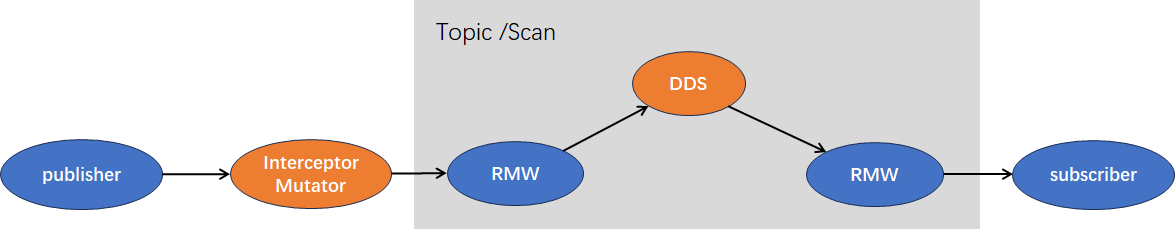
\includegraphics[width=15cm]{fuzz_msg_passing.png}
    \caption{本作品对不稳定网路的模拟机制}
    \label{pic:fmp}
\end{figure}

\subsubsection{多维度输入变异}

除了对上述ROS2内部通信消息进行变异,本作品同样也对传统程序输入进行变异,如输入
ROS2节点程序的命令、ROS2节点配置文件、用户交互数据等,见图\ref{pic:fmi}。通过多
个维度输入的变异,本作品可以高效地探索程序内部状态,更高效地尝试触发异常状态,检
测程序安全漏洞。

\begin{figure}[h]
    \centering
    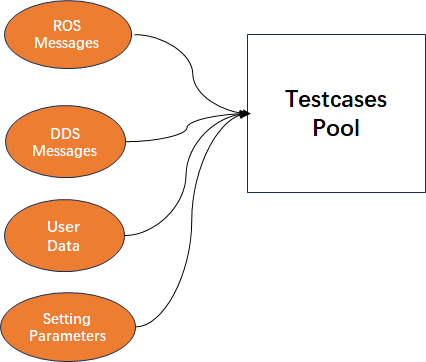
\includegraphics[width=7cm]{fuzz_multi_input.png}
    \caption{本作品针对多维度输入进行测试样例生成}
    \label{pic:fmi}
\end{figure}

\subsubsection{基于延迟插入的并发漏洞检测}

如背景知识一节所述,ROS2系统有典型的并发特征,在节点间是基于消息通信的多进程并发
模型,而在节点内则是基于共享内存的多线程并发模型。基于消息通信的并发模型容易出现
死锁等阻塞漏洞,基于共享内存的并发模型则容易出现数据竞争等并发漏洞,这两点导致了
基于ROS2的程序存在较多并发漏洞,对ROS系统漏洞的统计工作$^{[3]}$也证明了这一点。

针对这一点,本作品尝试通过延迟插入技术来检测并发漏洞,工作$^{[1]}$已说明这种方法
具有漏洞探测的便捷性与高效性。通过举例来解释该技术:在正常程序中,当对象A被使用
时,它不应被释放或已被释放,对对象A的释放操作应阻塞等待所有对对象A的使用操作结束
再执行;本作品会尝试在某些边界情况中(如系统频繁申请与释放资源时)在对象A的使用
操作前插入延迟,如图\ref{pic:fi}右图,如果此时对A的释放操作没有正确阻塞等待对象A
的使用完毕,而直接执行,就会造成严重的UAF内存错误,因为此时使用的对象A已经被释
放。

\begin{figure}[h]
    \centering
    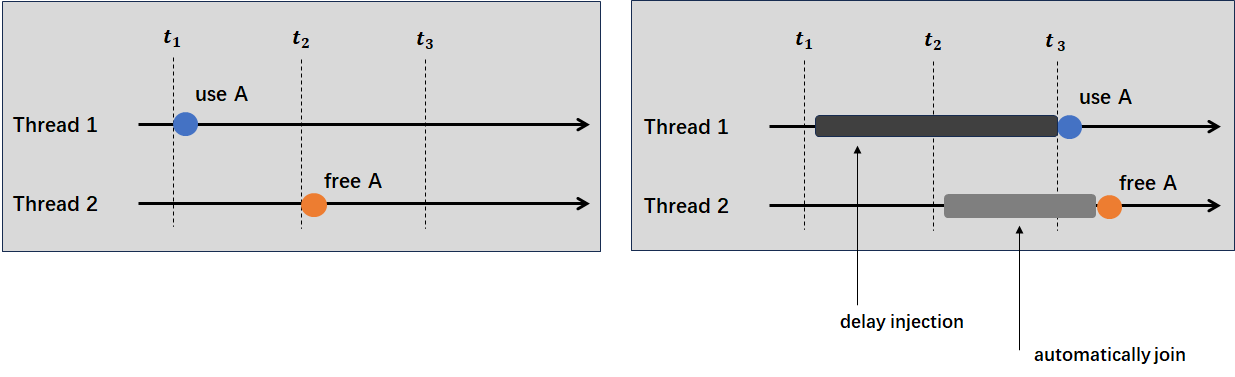
\includegraphics[width=15cm]{fuzz_delay_injection.png}
    \caption{延迟插入技术的探测漏洞原理}
    \label{pic:fdi}
\end{figure}

延迟插入技术可能拖慢整个程序的运行速度,所以具体插入位置需要谨慎选择。如前所
述,ROS2系统高度抽象化了各个子功能组件,将各个功能将回调函数绑定给执行器,执行器
负责监听事件并触发相应回调函数。统计$^{[3]}$显示这种线程模型是导致潜在数据竞争的
重要原因,由此,本作品基于LLVM框架对组件的回调函数前后插入检查点,如图
\ref{pic:fi}所示,对子线程可疑行为进行延迟插入,观察能否触发数据竞争漏洞。

\begin{figure}[h]
    \centering
    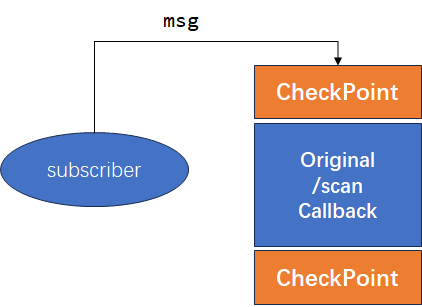
\includegraphics[width=7cm]{fuzz_instrumentation.png}
    \caption{延迟插入技术的实现}
    \label{pic:fi}
\end{figure}

\subsubsection{测试反馈}
模糊测试中,对“测试样例自动生成”的反馈指导质量直接影响了最终的测试效率,这种反馈
则取决于对被测程序的信息收集。传统被收集的信息包括调试信息、代码覆盖率等,这些信
息被认为反映了被测程序内部状态的变化。在此基础上,本系统创新性地利用我们魔改的
DDS中间件,对ROS2节点的流量进行分析,如图\ref{pic:ftm};同时利用插桩的检查点(如
图\ref{pic:fi})收集节点的功能组件回调函数执行信息,如执行时间、频率、传入的消息
内容等。这些额外信息更准确地反映了被测ROS2节点内部状态,指导我们更好地反馈生成新
测试样例,从而提高发掘漏洞的效率。

\begin{figure}[h]
    \centering
    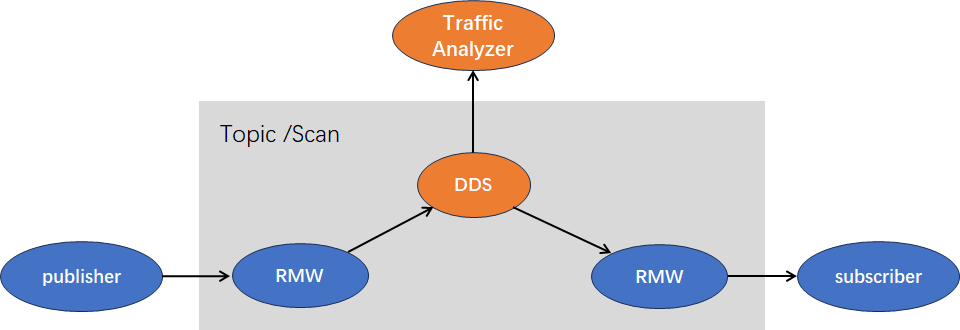
\includegraphics[width=15cm]{fuzz_traffic_monitor.png}
    \caption{利用替换的DDS中间件进行流量分析}
    \label{pic:ftm}
\end{figure}


\subsubsection{测试加速}

复杂机器人系统通常资源消耗大,对本地网络污染严重,进程管理复杂,这导致了对其测试
的低效性。测试人员或自动测试程序难以实现对测试行为的并行化:本地网络中存在的多个
同名程序实例(如多个Navigation2导航程序)会被其他实例的通信消息所干扰,这是因为
ROS2系统会共享同一个通信守护进程;一个基于ROS2的项目大多是多进程多线程的,每个进
程有独立进程组,关闭程序时容易遗留孤立进程,持续干扰整个ROS2环境。

针对这一情况,本作品创新性地使用Docker对不同测试实例进行进程、网络的隔离;搭配使
用随机化ROS2命名空间,提供更轻量化的网络隔离。通过这种方式,本作品可以充分利用电
脑性能进行并行化测试,变相大幅提升了自动测试效率,当然这也增加了本作品模糊测试程
序的开发难度。

\begin{figure}[h]
    \centering
    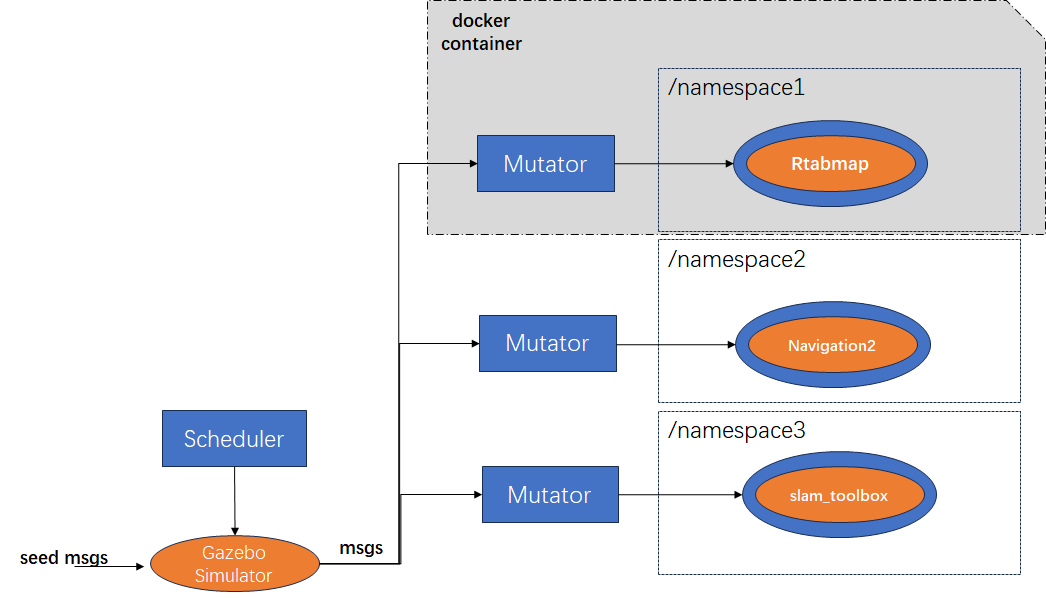
\includegraphics[width=15cm]{fuzz_container.png}
    \caption{测试的容器化与并行化}
    \label{pic:fc}
\end{figure}
